%--- Kapitel 10
\cleardoublepage
\chapter{Entwurfsmuster}
\label{sec:Kap-10}

Entwurfsmuster (engl. Design Patterns) rückten erstmals Mitte der 1990er Jahre mit dem Buch „Design Patterns: Elements of Reusable Object-Oriented Software“ \cite{gam95} von Erich Gamma, Richard Helm, Ralph Johnson und John Vlissides in den Fokus objektorientierter Softwareentwicklung.

Der Begriff Entwurfsmuster wird noch heute mit Erich Gamma verbunden, nicht nur weil er den alphabetisch "`kleinsten"' Nachnamen der vier Autoren hat und als Erstautor aufläuft, sondern weil die Arbeit an Mustern auf seine Dissertation \mbox{zurückgeht}.

Entwurfsmuster sind Schablonen \marginline{Entwurfsmuster vs. Architekturmuster} bewährter Lösungen für wiederkehrende und gleichartige Probleme. Im Unterschied zu Architekturmustern (Kap.~7.1.2) %todo (s.~Lektion~\ref{sec:Lektion-5})
operieren Entwurfsmuster auf der niedrigeren Ebene einzelner Klassen bzw. kleiner Module und beziehen sich nicht auf die großen Komponenten der Software. Entwurfsmuster beschreiben Lösungen auf einer abstrakten Ebene durch Diagramme und Text. Es handelt sich nicht um fertigen Programmcode, den man direkt ins eigene Programm kopieren könnte. Bestenfalls sind Quellcodebeispiele angegeben. Im Laufe der Jahre sind aber viele Entwurfsmuster für verschiedene Programmiersprachen im Rahmen von Bibliotheken oder Frameworks in Programmcode umgesetzt worden.

Warum nutzt \marginline{Wieder\-verwendung} man überhaupt Entwurfsmuster? Die Wiederverwendung von Teilen guter Entwürfe ist eine erfolgreiche Maßnahme um zu einem guten objekt\-orientierten Entwurf zu kommen. Entwickler mit großer Entwurfserfahrung profitieren häufig davon, dass sie in der Vergangenheit bereits mit ähnlichen Problemen konfrontiert waren, auf deren Lösungen sie bei neuen Softwareentwicklungsprojekten zurück\-greifen können. Durch Entwurfsmuster kann dieses Expertenwissen dokumentiert werden, und es kann auch von anderen Entwicklern genutzt werden. Erich Gamma und Kollegen schreiben in diesem Zusammenhang in ihrem Vorwort:

\sttpzitat{„Entwurfsmuster erfassen Problemlösungen, die im Laufe der Zeit gefunden wurden und sich weiterentwickelt haben. Es sind Entwürfe, auf die man üblicherweise nicht gleich von Anfang an kommt. Sie basieren auf vielen Entwurfsrevisionen und erneutem Programmieren, die Entwickler auf der Suche nach größerer Wiederverwendung und Flexibilität vorgenommen haben. Entwurfsmuster erfassen diese Lösungen auf konzentrierte und einfach anwendbare Weise.“ \cite[XV]{gam11}}{}

\pagebreak %%% für Druck

Das Buch \marginline{Kategorisierung} von Erich Gamma und Kollegen enthält 23 verschiedene Entwurfsmuster, die anhand ihres Einsatzzwecks in drei Kategorien eingeordnet sind: Erzeugende Muster, Strukturmuster und Verhaltensmuster. Erzeugende Muster zielen auf die Instanziierung, also den Prozess der Objekterzeugung. Strukturelle Muster beschäftigen sich mit der Zusammensetzung von Strukturen aus mehreren Klassen bzw. Objekten. Verhaltensmuster betrachten die Interaktion zwischen Objekten.

\vspace{2mm} %%% für Druck

Tabelle~\ref{table:entwurfsmuster_katalogisierung} zeigt die Einteilung der 23 Entwurfsmuster in diese Kategorien.

\vspace{\baselineskip} %%% für Druck

\begin{table}[ht]
	\setlength{\tabcolsep}{5pt}
	\renewcommand{\arraystretch}{1.5}
	
	\centering
	\small
	
	\begin{tabular}{ |c||p{2.7cm}|p{2.3cm}|p{3.0cm}| }
		\hline
		\multirow{2}{6em}{\centering Anwendungs\-bereich} & \multicolumn{3}{c|}{Aufgabe} \\
		\cline{2-4}
		& \multicolumn{1}{c|}{Erzeugung}
		& \multicolumn{1}{c|}{Struktur} & \multicolumn{1}{c|}{Verhalten} \\
		\hline
		\hline
		Klasse & Fabrikmethode & Adapter & Interpreter \newline Schablonenmethode \\
		\hline
		Objekt & Abstrakte Fabrik \newline Erbauer \newline Prototyp \newline Singleton
		& Adapter \newline Brücke \newline Dekorateur \newline Fassade \newline Fliegengewicht \newline Kompositum \newline Proxy
		& Befehl \newline Beobachter \newline Besucher \newline Iterator \newline Memento \newline Strategie \newline Vermittler \newline Zustand \newline Zuständigkeitskette \\
		\hline
	\end{tabular}
	\caption{Kategorisierung von Entwurfsmustern, nach \cite[14]{gam11}}
	\label{table:entwurfsmuster_katalogisierung}
\end{table}

\vspace{\baselineskip} %%% für Druck

Der Anwendungsbereich gibt an, ob sich ein Muster auf Klassen oder auf Objekte bezieht. Klassenmuster behandeln die Beziehungen zwischen Klassen und ihren Unter\-klassen. Im Mittelpunkt dieser Kategorie steht die Generalisierungsbeziehung. Die aus diesen Mustern resultierenden Strukturen sind statisch und können zur Laufzeit nicht mehr geändert werden. Objektmuster beziehen sich auf die Verbindungen zwischen Objekten, so dass die resultierenden Strukturen zur Laufzeit erstellt, geändert und wieder aufgehoben werden können. Sie verwenden hauptsächlich Assoziationen, aber auch die Generalisierung spielt eine gewisse Rolle.

\vspace{2mm} %%% für Druck

Das Muster Adapter kommt zweimal vor: einmal als Adapter auf Klassenebene und einmal als Muster auf Objektebene.

\vspace{2mm} %%% für Druck

Für die Wiederverwendbarkeit eines Entwurfsmusters ist eine übersichtliche und verständliche Dokumentation wichtige Voraussetzung. Diese beschreibt das grundsätzliche Entwurfsproblem, den Anwendungskontext und eine Lösungsstruktur. 

\clearpage %%% für Druck

Ein Entwurfsmuster wird hierfür üblicherweise nach einem Schema folgender oder ähnlicher Art dokumentiert:

\begin{addmargin}[25pt]{25pt}
\begin{description}
	\setlength{\itemsep}{2mm} %%% für Druck
	
	\item[Zweck] des Musters
	\item[Synonyme,] unter denen das Muster auch bekannt ist
	\item[Motivation] Einordnung, Zweck und Einsatzmotive, Fallbeispiele
	\item[Anwendbarkeit] Indikatoren für den Einsatz des Musters
	\item[Struktur] des Musters
	\item[Beteiligte] Klassen und/oder Objekte
	\item[Zusammenspiel] der beteiligten Klassen bzw. Objekte
	\item[Konsequenzen] Vor- und Nachteile
	\item[Implementierung] beispielhafter Quellcode
	\item[Praxiseinsatz] Beispiele und Nachweise über den erfolgreichen Einsatz
	\item[Querverweise] und Abgrenzungen zu ähnlichen Mustern
\end{description}
\end{addmargin}

In dem Buch „Design Patterns mit Java“ von Olaf Musch \cite{mus21} finden Sie für alle der ursprünglich von Gamma und Kollegen zusammengestellten Muster ausführliche Beschreibungen mit Lebensweltbeispielen für deren Einsatzzweck sowie Quellcodebeispielen für deren Umsetzung in Java.

Die folgenden Abschnitte~\ref{sec:Kap-10.1} bis \ref{sec:Kap-10.3} stellen jeweils beispielhaft ein Entwurfsmuster der drei Entwurfsmusterkategorien vor. Sie basieren auf der vorherigen Version des Kurstextes von Hans-Werner Six und Mario Winter, der sich stark an der Darstellung in \cite{gam95} orientierte. 

% 10.1
\clearpage
\section{Erzeugende Muster}
\label{sec:Kap-10.1}

\textit{Erzeugende Muster} abstrahieren den Instanziierungsprozess und machen eine Anwendungssoftware unabhängig davon, wie ihre Objekte erzeugt und zusammen\-gesetzt werden. Erzeugende Muster werden dann wichtig, wenn die Software nach einigen Änderungen immer mehr auf die Komposition vieler Objekte als auf wenige Generalisierungshierarchien aufbaut.
%Im Verlauf der Evolution von Anwendungssystemen wird es nämlich erfahrungsgemäß immer wichtiger, den Fokus von festverdrahteten komplexen Schnittstellen hin zu einer Menge möglichst schlanker, orthogonaler Schnittstellen zu verschieben, aus denen die komplexeren Schnittstellen zusammengesetzt werden können.
Die Erzeugung von Objekten mit bestimmtem Verhalten erfordert dann mehr als die einfache Instanziierung einer Klasse.

In \cite{gam95} werden fünf erzeugende Muster vorgestellt, die teilweise aufeinander aufbauen:

\begin{description}
	\setlength{\itemsep}{2mm} %%% für Druck
	
	\item[\textit{Abstrakte Fabrik}] (abstract factory) bietet eine Schnittstelle zum Erzeugen von Familien verwandter oder voneinander abhängiger Objekte, ohne ihre konkreten Klassen zu benennen.
	\item[\textit{Einzelstück}] (singleton) stellt sicher, dass von einer Klasse nur eine einzige Instanz existiert, und bietet einen globalen Zugriffsmechanismus auf diese Instanz an.
	\item[\textit{Erbauer}] (builder) trennt den Aufbau eines komplexen Objekts von seiner Darstellung, so dass mittels desselben Konstruktionsvorgangs verschiedene Repräsentationen erzeugt werden können.
	\item[\textit{Fabrikmethode}] (factory method) definiert eine Schnittstelle zur Erzeugung eines Objekts, aber überlässt die Entscheidung, welche Klasse zu instanziieren ist, den Unterklassen. Die Fabrikmethode ermöglicht einer Klasse, die Instanzi\-ierung ihren Unterklassen zu überlassen.
	\item[\textit{Prototyp}] (prototype) spezifiziert die Art der zu erzeugenden Objekte über eine \mbox{exemplarische} Instanz und erzeugt neue Objekte durch Kopieren dieser Instanz.
\end{description}

\vspace{\baselineskip}
\textcolor{FernUni-MI-green}{\noindent\rule[1ex]{\textwidth}{2pt}}\\
{\Large \textcolor{FernUni-MI-green}{\textsc{Abstrakte Fabrik (Abstract Factory)}}}\\
\textcolor{FernUni-MI-green}{\noindent\rule[1ex]{\textwidth}{2pt}}

\begin{description}
	\setlength{\itemsep}{2mm} %%% für Druck
	
	\item[Zweck] Bietet eine Schnittstelle zum Erzeugen von Familien verwandter oder voneinander abhängiger Objekte, ohne ihre konkreten Klassen zu benennen.
	\item[Motivation] Angenommen, eine Klassenbibliothek zur Unterstützung grafisch-
	\linebreak %%% für Druck
	interaktiver Benutzungsschnittstellen soll mehrere „Look\&Feel“-Standards unterstützen, wobei unterschiedliche Standards unterschiedliches Aussehen und Verhalten von graphischen Bedienungselementen wie \zb Scrollbar oder 
	\linebreak %%% für Druck
	Fenstern festlegen. Um unter verschiedenen solcher Standards lauffähig zu sein, darf eine Anwendungssoftware die benutzten Bedienelemente nicht statisch zur Kompilierungszeit festlegen, sondern muss dynamisch zur Laufzeit die ge\-eigneten Elemente auswählen und entsprechende Klassen instanziieren.
	
\pagebreak %%% für Druck

	Wir können dieses Problem lösen, indem wir in einer abstrakten Klasse eine Schnittstelle definieren, welche Operationen zur Erzeugung jedes Bedien\-elements zur Verfügung stellt. Für jeden zu unterstützenden Standard bilden wir eine (konkrete) Unterklasse dieser abstrakten Klasse. Zusätzlich definieren wir für jedes der Bedienelemente eine abstrakte Klasse, von der für jeden Standard eine Unterklasse zur Realisierung des entsprechenden Elements abgeleitet wird. Die Erzeugungsoperation für ein Bedienelement liefert nun bei jedem Aufruf eine neue Instanz dieses Bedienelements, aber je nach gewählter konkreter Fabrik-Unterklasse eine Instanz der Element-Unterklasse, die das Bedienelement für den entsprechenden Standard realisiert.
	
	Anwendungsprogramme, welche die Elemente der Benutzungsschnittstelle verwenden erzeugen diese ausschließlich über die Schnittstelle der abstrakten Klasse und haben keinerlei Kenntnis von der konkreten Realisierung der Elemente für einen bestimmten Benutzungsschnittstellen-Standard.
	\item[Anwendbarkeit] Man verwendet das Muster Abstrakte Fabrik unter folgenden
	\linebreak %%% für Druck
	Bedingungen:
	\begin{itemize}
		\item 	Die Anwendungssoftware soll unabhängig davon sein, wie bestimmte 
		\linebreak %%% für Druck
		Objekte (im Muster „Produkte“ genannt) erzeugt, zusammengesetzt und präsentiert werden.
		\item 	Die Anwendungssoftware soll für eine von mehreren Familien von Produkten konfigurierbar sein.
		\item 	Nur Produkte aus einer Familie können zusammenarbeiten.
		\item 	Eine Bibliothek wiederverwendbarer Klassen soll nur über die Schnittstellen verfügbar gemacht werden.
	\end{itemize}
	
	\item[Struktur] Abbildung~\ref{fig:muster_abstrakte_fabrik} zeigt die allgemeine Struktur des Musters Abstrakte
	\linebreak %%% für Druck
	Fabrik.
	
	\begin{figure}[h!]
		\centering
		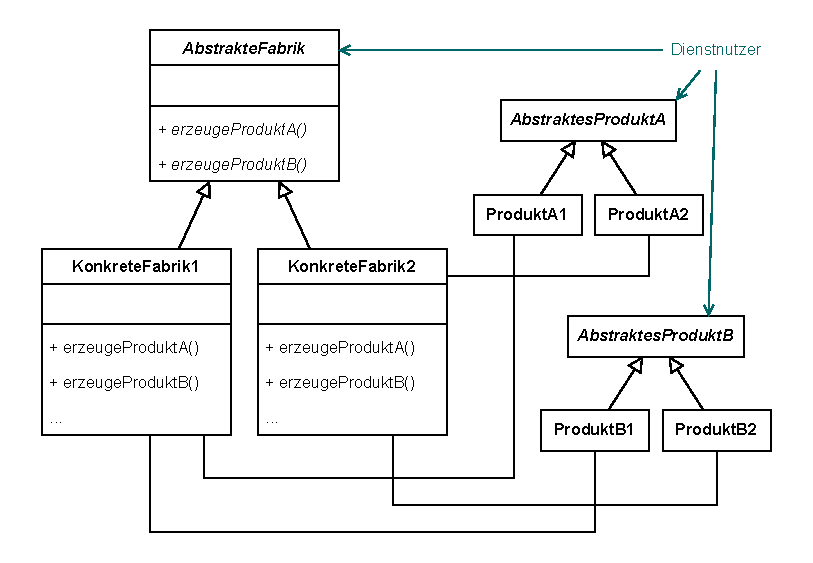
\includegraphics[scale=1.0]{Bilder/Kapitel-10/muster_abstrakte_fabrik.pdf}
		\caption{Allgemeine Struktur des Musters Abstrakte Fabrik}
		\label{fig:muster_abstrakte_fabrik}
	\end{figure}	
	
	\vspace{1mm} %%% für Druck
	
	\item[Konsequenzen] Das Muster Abstrakte Fabrik hat folgende Vor- und Nachteile:
	\begin{itemize}
		\item 	Es isoliert konkrete Klassen und hilft die von der Anwendungssoftware instanziierbaren Klassen zu kontrollieren. Da eine Fabrik die Verantwortlichkeit und den Prozess der Erzeugung von Produkt\-instanzen verkapselt, isoliert sie die Anwendungssoftware von den realisierenden Klassen. Klassennamen der konkreten Produktklassen tauchen somit nicht in den Klassen der Anwendungssoftware auf. Diese manipuliert Produkt\-instanzen nur über die Schnittstelle der abstrakten Produktklassen.
		\item 	Es vereinfacht den Austausch ganzer Produktfamilien, da die Klasse einer konkreten Fabrik nur einmal explizit angesprochen wird, nämlich am Ort ihrer Instanziierung.
		\item 	Die von der Anwendungssoftware verwendete Produktfamilie kann einfach durch Angabe einer anderen konkreten Fabrik geändert werden. 
		\item 	Es erzwingt die Konsistenz der von der Anwendungssoftware benutzten Produkte, wenn zu einem bestimmten Zeitpunkt nur genau eine Instanz (einer Unterklasse) der Klasse \sttpUMLText{AbstrakteFabrik} existieren darf. Dies ist insbesondere dann wichtig, wenn die Produkte aus unterschiedlichen Familien nicht untereinander kompatibel sind.
		\item 	Es erschwert die Hinzunahme neuer Produkte, da jede abstrakte Fabrik eine Operation zur Erzeugung jedes Produkts einer Familie definiert. Für jedes neue Produkt müssen also diese Schnittstelle und eine Implementierung in allen konkreten Unterklassen der abstrakten Fabrik sowie des abstrakten Produkts eingeführt werden.
	\end{itemize}
\end{description}


% 10.2
\clearpage
\section{Strukturmuster}
\label{sec:Kap-10.2}

\textit{Strukturmuster} beschreiben, wie Klassen bzw. ihre Instanzen zu größeren Strukturen zusammengesetzt werden können. In \cite{gam95} finden wir folgende sieben Strukturmuster:

\begin{description}
	\setlength{\itemsep}{2mm} %%% für Druck
	
	\item[\textit{Adapter}] (adapter) wandelt die Schnittstelle (gegebener) dienstleistender Klassen so um, dass dienstnutzende Klassen sie verwenden können.
	\item[\textit{Brücke}] (bridge) entkoppelt eine Abstraktion von ihrer Implementierung, damit beide unabhängig voneinander verändert werden können.
	\item[\textit{Dekorateur}] (decorator) heftet dynamisch zusätzliche Verantwortlichkeiten (Operationen) an ein Objekt. Dekorateure basieren auf Dienstnutzungen und stellen für die Funktionalitätserweiterung eine flexible Alternative zur Generalisierung dar.
	\item[\textit{Fassade}] (facade) stellt eine einheitliche Schnittstelle für eine Menge von Schnitt\-stellen zur Verfügung und führt eine Strukturierungsebene oberhalb von Klassen ein.
	\item[\textit{Fliegengewicht}] (flyweight) benutzt wenige (komplexe) Objekte mehrfach (shared objects), um eine große Anzahl kleiner Objekte effizient handhaben zu können.
	\item[\textit{Kompositum}] (composite) ermöglicht den einheitlichen Zugriff auf die Elemente hierarchisch strukturierter Objektstrukturen und bietet dafür eine Schnittstelle, mit der individuelle Objekte (Blätter eines Baums) und Kompositionen (innere Knoten) gleichbehandelt werden können.
	\item[\textit{Proxy}] (proxy) stellt über ein stellvertretendes Objekt eingeschränkte Zugriffe auf das eigentliche Objekt zur Verfügung.
\end{description}

\vspace{\baselineskip} %%% für Druck

\vspace{\baselineskip}
\textcolor{FernUni-MI-green}{\noindent\rule[1ex]{\textwidth}{2pt}}\\
{\Large \textcolor{FernUni-MI-green}{\textsc{Fassade}}}\\
\textcolor{FernUni-MI-green}{\noindent\rule[1ex]{\textwidth}{2pt}}

\begin{description}
	\setlength{\itemsep}{2mm} %%% für Druck
	
	\item[Zweck] Stellt eine einheitliche Schnittstelle für eine Menge von Schnittstellen zur Verfügung und führt eine Strukturierungsebene oberhalb von Klassen ein.
	\item[Motivation] Ein häufiges Ziel im Entwurf ist die Minimierung der Abhängigkeiten zu einer Gruppe von eng zusammenarbeitenden Klassen (einem Cluster). Ein Weg zur Erreichung dieses Zieles ist der Einsatz eines Fassaden-Objekts, welches eine einfache Schnittstelle zu der Funktionalität des Clusters anbietet (Abb.~\ref{fig:muster_fassade}).
	
\clearpage %%% für Druck

\vspace*{2mm} %%% für Druck

	\begin{figure}[h!]
		\centering
		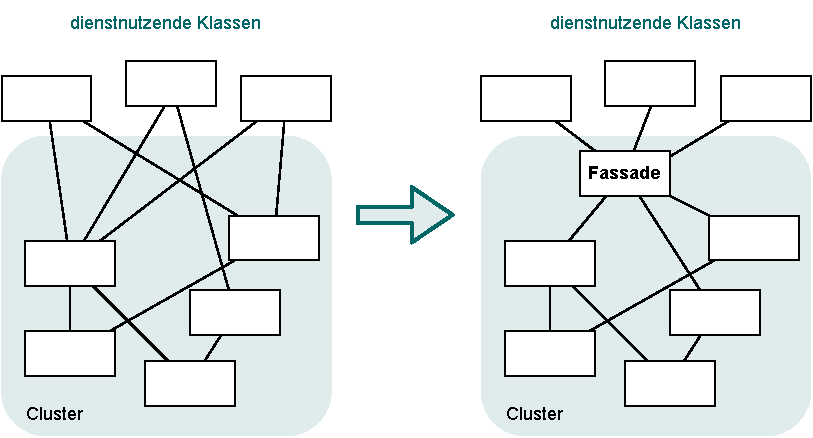
\includegraphics{Bilder/Kapitel-10/muster_fassade.pdf}
		\caption{Grundstruktur des Fassade-Musters}
		\label{fig:muster_fassade}
	\end{figure}

	\item[Anwendbarkeit] Man verwendet das Muster Fassade unter folgenden Bedingungen:
	\begin{itemize}
		\item 	Ein komplexes Cluster soll eine einfache Schnittstelle erhalten. Cluster werden häufig im Lauf ihrer Entwicklung komplexer. Die meisten Muster führen durch ihre Anwendung zu mehr und kleineren Klassen. Die Anwendung des Musters Fassade macht die Cluster besser wiederverwendbar und adaptierbar, gleichzeitig wird ihre Nutzung aber für jene schwieriger, die keine Adaptierung für ihre Aufgabenstellung benötigen. Eine Fassade bietet eine einfache Standardsicht des Clusters an, die für die meisten Dienstnutzer ausreicht.
		\item 	Es existieren viele Abhängigkeiten zwischen den Dienstnutzern und den Implementierungsklassen einer Abstraktion. Man verwendet das Muster Fassade, um die Abhängigkeiten zwischen den Dienstnutzern und dem Cluster in der Fassaden-Klasse zu konzentrieren und dadurch seine Unabhängigkeit und Portabilität zu erhöhen.
		\item 	Dienstnutzer, die eine größere Flexibilität oder umfangreichere Funktionalität benötigen, müssen unter Umgehung der Fassade auf einzelne Klassen des Clusters zurückgreifen.
	\end{itemize}
	
	\item[Zusammenspiel] Dienstnutzer kommunizieren mit dem Cluster, indem sie Methoden der Fassade aufrufen, welche die Aufrufe an die entsprechenden Objekte des Clusters weiterleiten. Obwohl die Clusterobjekte die eigentliche Arbeit leisten, muss die Fassade eventuell selbst Arbeit leisten, um ihre Schnittstelle in die Schnittstellen der Clusterobjekte zu übersetzen. Die Dienstnutzer der Fassade können auf alle oder ausgewählte Objekte des Clusters direkt zugreifen, indem sie vom Fassadenobjekt eine Referenz auf diese Objekte anfordern.
	\item[Konsequenzen] Das Muster Fassade hat folgende Vorteile:
	\begin{itemize}
		\item 	Es trennt Dienstnutzer von Objekten eines Clusters und reduziert dadurch die Anzahl der Objekte, mit denen der Dienstnutzer zu tun hat. Dadurch wird die Benutzung des Clusters einfacher.
		\item 	Es reduziert die Kopplung zwischen dem Dienstnutzer und den Objekten eines Clusters.
		\item 	Es verhindert nicht die direkte Nutzung der Objekte des Clusters durch Anwendungen, falls dies notwendig ist. Man kann zwischen einer ein\-fachen Benutzung und vollständigem Funktionsumfang wählen.
	\end{itemize}

	\item[Implementierung] Eine Möglichkeit die Kopplung zwischen Dienstnutzern und \linebreak %%% für Druck
	Cluster weiter zu reduzieren, ist die Realisierung der Klasse Fassade als abstrakte Klasse oder Interface. So ist der Dienstnutzer nicht an eine konkrete Implementierung eines Clusters gebunden.
	
	Ein Cluster kann in Java als Paket realisiert werden, wobei die Fassaden-Klasse und ausgewählte Klassen des Clusters außerhalb des Paketes sichtbar sind, alle anderen Klassen des Clusters aber nur innerhalb des Pakets.	
\end{description}

% 10.3
\clearpage
\section{Verhaltensmuster}
\label{sec:Kap-10.3}

Einzelne Objekte alleine sind meistens uninteressant. Erst Objektgeflechte, in denen jedes Objekt seine speziellen Fähigkeiten anderen Objekten zur Verfügung stellt oder auf die Fähigkeiten anderer Objekte zurückgreift, bilden die Essenz einer objektorientierten Anwendungssoftware. \textit{Verhaltensmuster} beschreiben, wie eine gegebene Funktionalität auf Verantwortlichkeiten unterschiedlicher Klassen bzw. ihrer Instanzen abgebildet werden kann, und bilden die größte Gruppe der in \cite{gam95} katalogisierten Entwurfsmuster.

Zusätzlich zu den in Strukturmustern dargestellten reinen Klassen- bzw. Objektstrukturen beschreiben Verhaltensmuster auch den Nachrichtenaustausch innerhalb solcher Strukturen. Zwei dieser Muster (Schablonenmethode und Interpreter) verwenden die Generalisierung, die anderen die Aggregation bzw. Komposition von Klassen, um eine gegebene Funktionalität zu zerlegen. 

\begin{description}
	\setlength{\itemsep}{2mm} %%% für Druck
	
	\item[\textit{Befehl}] (command) verkapselt Operationsaufrufe bzw. Nachrichten, sodass Dienstnutzungen parametrisiert, aneinandergereiht, aufgezeichnet oder aber später rückgängig gemacht (undo) werden können.
	\item[\textit{Beobachter}] (observer) definiert eine 1:m-Abhängigkeit zwischen Objekten, damit Zustandsänderungen eines Objekts an andere gemeldet und diese aktualisiert werden können.
	\item[\textit{Besucher}] (visitor) repräsentiert eine Operation, welche auf die einzelnen Elemente einer Objektstruktur angewendet wird und ermöglicht die Definition einer neuen Operation, ohne die Klassen, auf deren Instanzen die Operation arbeitet, ändern zu müssen.
	\item[\textit{Interpreter}] (interpreter) interpretiert Sätze in einer gegebenen Sprache aufbauend auf einer Grammatikrepräsentation mittels der Generalisierung.
	\item[\textit{Iterator}] (iterator) stellt den Zugriff auf die einzelnen Elemente einer Struktur zur Verfügung, ohne die Implementierung der Struktur offenzulegen.
	\item[\textit{Schablonenmethode}] (template method) definiert das Grundgerüst eines Algorithmus, aber überlässt Unterklassen die Implementierung von Details. Unter\-klassen können die variablen Teile des Algorithmus unterschiedlich implementieren, das Grundgerüst des Algorithmus bleibt aber fest.
	\item[\textit{Memento}] (memento) erfasst und speichert den Zustand eines Objekts, ohne das Geheimnisprinzip zu durchbrechen, und ermöglicht die spätere Wieder\-her\-stellung dieses Zustands.
	\item[\textit{Strategie}] (strategy) definiert eine Familie von Algorithmen, verkapselt sie und macht sie austauschbar. Das Muster ermöglicht die Variation der Implementierung einer Operation unabhängig von den aufrufenden Objekten.

\pagebreak %%% für Druck

	\item[\textit{Vermittler}] (mediator) definiert ein Objekt, welches die Interaktionen mehrerer anderer Objekte in sich verkapselt. So wird die Kopplung zwischen den anderen Objekten abgeschwächt und die unabhängige Änderung einzelner Inter\-aktionen ermöglicht.
	\item[\textit{Zustand}] (state) erlaubt einem Objekt, sein Verhalten abhängig vom Zustand zu verändern, sodass es als Instanz einer anderen Klasse erscheint.
	\item[\textit{Zuständigkeitskette}] (chain of responsibility) vermeidet die Kopplung eines Dienstnutzers an mehrere Dienstleister, indem die entsprechenden Nachrichten mehreren „aneinandergereihten“ Dienstleistern der Reihe nach angeboten werden.
\end{description}

\vspace{\baselineskip} %%% für Druck

\vspace{\baselineskip}
\textcolor{FernUni-MI-green}{\noindent\rule[1ex]{\textwidth}{2pt}}\\
{\Large \textcolor{FernUni-MI-green}{\textsc{Iterator}}}\\
\textcolor{FernUni-MI-green}{\noindent\rule[1ex]{\textwidth}{2pt}}

\vspace{2mm} %%% für Druck

\begin{description}
	\setlength{\itemsep}{2mm} %%% für Druck
	
	\item[Zweck] Stellt den Zugriff auf die einzelnen Elemente einer Struktur zur Verfügung, ohne die Implementierung der Struktur offenzulegen.
	\item[Motivation] Ein Behälterobjekt, wie \zb eine Liste, sollte Operationen zum Zugriff auf ihre Elemente zur Verfügung stellen, ohne dass die interne Implementierung sichtbar wird. Es kann sein, dass die Liste auf unterschiedliche Weisen durchlaufen werden soll (\zb vorwärts und rückwärts), oder dass mehrere Durchläufe parallel stattfinden müssen.
	Das Iterator-Muster ermöglicht dies, indem die Verantwortung für den Zugriff und das Durchlaufen des Behälters aus dem Behälterobjekt in ein sog. \textit{Iteratorobjekt} verschoben wird. Das Iteratorobjekt merkt sich die aktuelle Position des Durchlaufs bzw. kennt die bereits besuchten Objekte. Der Zugriff auf das Behälterobjekt und auf das Iterator\-objekt erfolgt über Interfaces, damit die Implementierung für den Dienstnutzer verborgen und dadurch austauschbar ist.
	\item[Anwendbarkeit] Man benutzt das Iterator-Muster,
	\begin{itemize}
		\item 	um auf die Elemente eines Behälterobjekts zuzugreifen, ohne die interne Realisierung zu kennen;
		\item 	um mehrere parallele Durchläufe durch den Behälter zu ermöglichen;
		\item 	um ein einheitliches Interface zum Durchlaufen verschiedener Behälterstrukturen zu verwenden.
	\end{itemize}
	\item[Struktur] Abb.~\ref{fig:muster_iterator} zeigt die allgemeine Struktur des Iterator-Musters.

	\begin{figure}[h!]
		\centering
		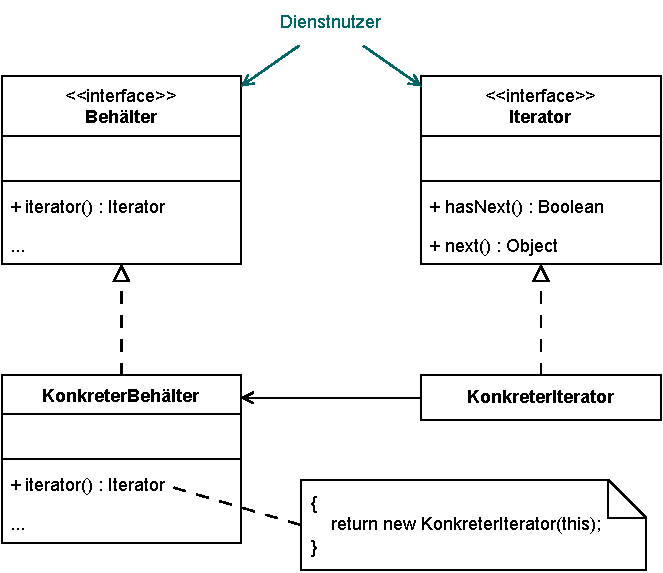
\includegraphics[scale=1.0]{Bilder/Kapitel-10/muster_iterator.pdf}
		\caption{Allgemeine Struktur des Iterator-Musters}
		\label{fig:muster_iterator}
	\end{figure}

	\item[Beteiligte] ~
	\begin{itemize}
		\item 	Das Interface Iterator definiert eine Schnittstelle mit Operationen zum sequentiellen Zugriff auf die Elemente eines Behälterobjekts.
		\item 	Die Klasse \sttpUMLText{KonkreterIterator} implementiert das Iterator-Interface und speichert den aktuellen Zustand des Behälterdurchlaufs.
		\item 	Das Interface \sttpUMLText{Behälter} definiert (neben den typischen Behälteropera\-tionen) eine Operation zum Erzeugen eines Iteratorobjekts.
		\item 	Die Klasse \sttpUMLText{KonkreterBehälter} implementiert die iterator()-Operation aus dem Behälter-Interface und liefert ein zum Behälter passendes 
		\linebreak %%% für Druck
		Iteratorobjekt.
	\end{itemize}
	
	\item[Zusammenspiel] Das konkrete Iteratorobjekt merkt sich das aktuelle Element des Behälters und kann das nächste Objekt des Durchlaufs berechnen.
	\item[Konsequenzen] Das Iterator-Muster hat folgende Vorteile:
	\begin{itemize}
		\item 	Es ermöglicht verschiedene Arten eines Behälterdurchlaufs. Beispiels\-weise kann eine Baumstruktur in verschiedenen Reihenfolgen (\zb in-order, pre-order oder post-order) durchlaufen werden. Iteratoren machen es einfach, den Durchlaufalgorithmus auszutauschen: Man tauscht einfach das Iteratorobjekt gegen ein anderes aus, das ebenfalls das Iterator-Interface implementiert.
		\item 	Iteratoren vereinfachen die Schnittstelle von Behältern, da anstelle der Durchlaufoperationen nur noch eine Operation erforderlich ist, die den Iterator erzeugt.
		\item 	Da ein Iterator den aktuellen Durchlaufzustand speichert, können mehrere Durchläufe durch einen Behälter parallel stattfinden.
	\end{itemize}	
	
\end{description}
	

% 10.4
\clearpage
\section{Entwurfsmuster vs. Frameworks vs. Bibliotheken}
\label{sec:Kap-10.4}

Es ist nicht sinnvoll, in jedem Softwareentwicklungsprojekt den Programmcode aus den basalen Elementen der Programmiersprache von Grund auf neu zu schreiben. Im Idealfall sollten sich die Entwickler in einem Projekt stattdessen auf diejenigen Aspekte konzentrieren können, die für das jeweilige Projekt spezifisch sind und für alles andere von bereits geleisteten Arbeiten und Erfahrungen profitieren.

Die Verwendung von Entwurfsmustern ist solch eine Möglichkeit, von Erfahrungen zu profitieren. Doch auch weniger abstrakte Vorarbeiten in Form von schon vor\-ge\-fertigten Codebausteinen und Programmlogiken werden verwendet, um die benötigte Software in der gewünschten Qualität zu entwickeln. \textit{Bibliotheken} und \textit{Frameworks} sind Möglichkeiten für die eigene zu erstellende Software auf bewährte, gut getestete und in zahlreichen anderen Entwicklungsprojekten eingesetzte Bestandteile zurückzugreifen.

Bibliotheken \marginline{Bibliotheken} (auch Klassenbibliotheken oder Programmbibliotheken genannt) bestehen aus wiederverwendbaren Klassen, die nützliche und allgemeine Funktionalitäten zur Verfügung stellen, die aus dem eigenen Programmcode heraus aufgerufen werden können. Viele Programmiersprachen bringen bereits eigene Bibliotheken mit. So besteht die Java-Standardbibliothek aus mehreren tausend Klassen mit Operationen für viele Problemstellungen. Eine Bibliothek ist kein eigenständig lauf{}fähiges Programm. Sie ist eine Sammlung von schon in Quellcode umgesetzten Funktionalitäten, von denen Entwickler die für ihr Programm benötigten Teile einsetzen. Die Verwendung einer Bibliotheksklasse bringt natürlich nur dann die genannten Vorteile, wenn sie genau zu der Anforderung passt und vom Programmierer genau so verwendet wird, wie vom Ersteller vorgesehen. Andernfalls steigt das Risiko für fehlerhafte Software sogar, wenn fremde Klassen blind zusammengewürfelt werden.
 
Beim Einsatz von Bibliotheken entwerfen die Entwickler das Grundgerüst für ihr Programm (Klassen und ihre Beziehungen, Ablauf des Programms) selber, evtl. ausgerichtet auf abstrakt beschriebene Entwurfsmuster, und binden die durch eine Bibliothek zur Verfügung gestellten Funktionalitäten an den geeigneten Stellen ihres Programmgerüsts ein.

Bei der Arbeit \marginline{Frameworks} mit Frameworks geht man den umgekehrten Weg. Ein Framework liefert bereits das Grundgerüst für das Programm. Die Entwickler müssen innerhalb dieses Grundgerüstes noch die Aspekte programmieren, die spezifisch für ihre Software sind (wobei auch an dieser Stelle aus Bibliotheken eingebunden werden kann).

Um es noch etwas komplizierter zu machen: In der Regel basieren Frameworks auf einer spezifischen Zusammenstellung mehrerer Entwurfsmuster. Und eigentlich ist es insofern die Kombination der verwendeten Entwurfsmuster, die das Programmgerüst bestimmt und das Framework nur die Umsetzung dieser Kombination. Des Weiteren können auch Bibliotheken auf Entwurfsmustern basieren, und wenn man diese einbindet, hat das evtl. doch Auswirkungen auf das eigene Programmgerüst.


% 10.5
\clearpage
\section{Kommentierte Literatur}
\label{sec:Kap-10.5}


\sttpKommLitItem{Gamma/Helm/Johnson/Vlissides}{1995}{Design Patterns}{gam95}{}{}
{Das Originalbuch zu Entwurfsmustern. Es ist in zahlreichen Neuauflagen und Übersetzungen erschienen. Mittlerweile gibt es zwar einige weitere anerkannte Entwurfsmuster und zusätzliche Kategorien, die Arbeiten von Gamma und Kollegen haben aber auch heute noch einen hohen Stellenwert.} 

\sttpKommLitItem{Musch}{2021}{Design Patterns mit Java}{mus21}{}{}
{Sehr strukturierte und auch für Anfänger im Thema Entwurfsmuster gut verständ\-liche Beschreibung der ursprünglich von \cite{gam95} vorgestellten Entwurfsmuster. Jedes Muster wird anhand eines Lebensweltbeispiels eingeführt und seine Einsatzzwecke vorgestellt. Mögliche Umsetzungen in Programmcode werden mit Java gezeigt.}

\sttpKommLitItem{Broy/Kuhrmann}{2021}{Einführung in die Softwaretechnik}{bro21}{}{}
{Kapitel 10 behandelt Entwurfsmuster. Dort wird auch deren Abgrenzung zu 
\linebreak %%% für Druck
Architekturmustern, Frameworks und Bibliotheken thematisiert.}




